% Management Summary

\begingroup
\let\clearpage\relax
\let\cleardoublepage\relax
\let\cleardoublepage\relax

\chapter*{Management Summary}
\label{management-summary}

%---------------------------------------------------
\subsection*{Situation}\label{introduction}

Digital mapping is moving towards vector tiles to create more interactive and resolution independent cartography. Instead of delivering the image of the map to the client, the vector representation of the data is sent to the map client.\\

Several vector tile providers such as Mapbox open the process to create vector tiles but still own the vector tile data. Developers and cartographers who want to be independent from 3rd party services or have limited internet access in their applications require free and global vector tiles to create the next generation of map applications.

\begin{figure}[H]
\centering
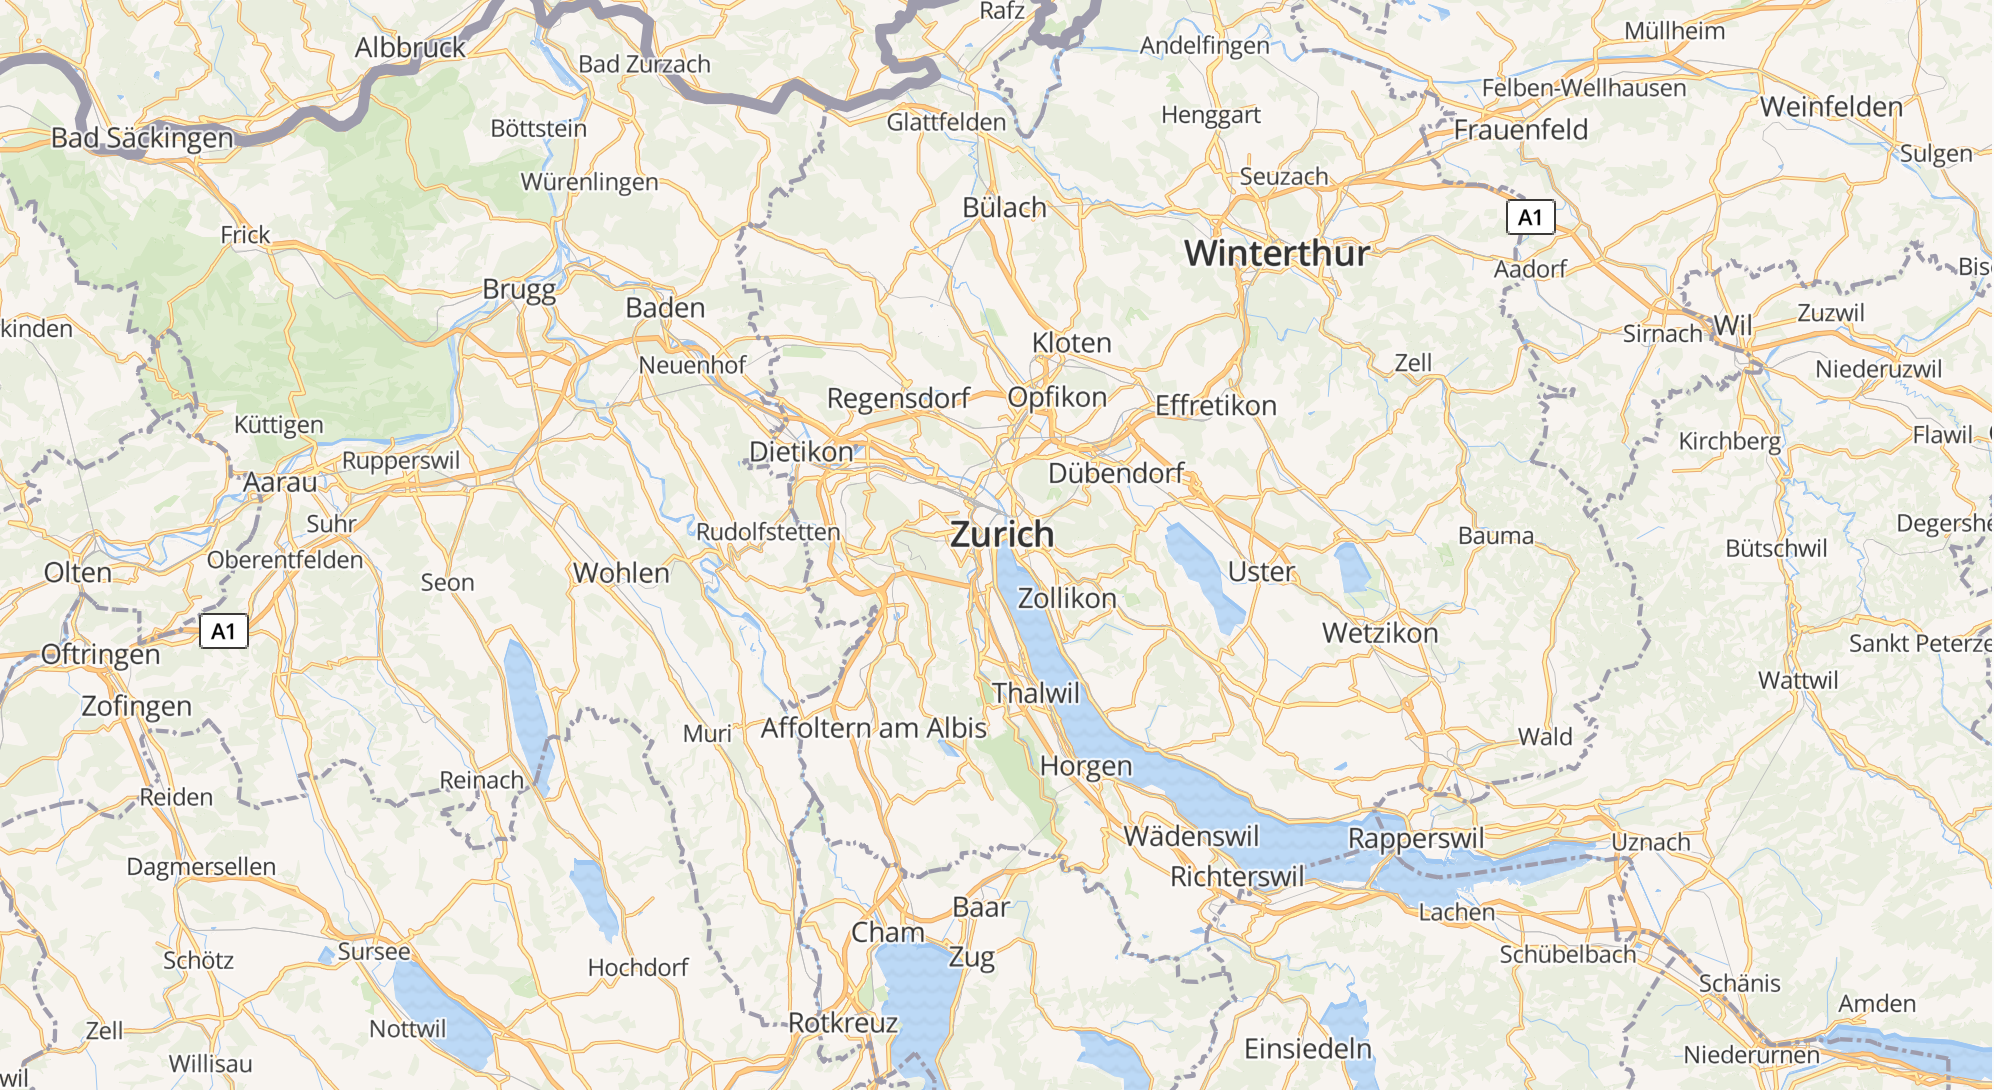
\includegraphics[width=\textwidth]{images/osm_bright}
\caption*{Map rendered from \osmvt{} vector tiles}
\end{figure}

%---------------------------------------------------
\subsection*{Approach}

The \osmvt{} project strives to push mapping forward by providing free and high quality vector tiles with no strings attached. To make developers independent from the providers
the vector tiles can be downloaded and hosted using a tileserver of their choice. This approach differs from all other vector tile providers and will enable new possibilities for desktop and mobile developers creating offline map applications.\\

The process to improve \osmvt{} is completely open and the feedback and requirements of the
community have been the cornerstone for improving the project with most feature requests and
bug reports coming from actual users.

%---------------------------------------------------
\subsection*{Result}

The result of this thesis are downloadable vector tiles for the entire world and extracts for over 200 countries and 600 cities provided on the project website \url{http://osm2vectortiles.org}. The vector tiles are compatible with the newest Mapbox Streets v7 vector tiles which allows people to use their visual styles created with Mapbox Studio together with OSM2VectorTiles.\\

The workflow to create the vector tiles is available for everyone to use and is meant to be adapted by other projects. The workflow can be scaled linearly by adding more worker machines and is a unique approach to rendering offline vector tiles with global coverage.\\

The vector tiles can be kept up to data by continuously applying the latest \osm{} changes and rerendering only the parts of the planet that are affected by those changes. This enables to provide downloadable vector tiles but still keep the data up to date.\\

The \osmvt{} project is already used in several real world projects and by pushing the project further the result of this thesis is a living open source project that hopefully will survive this bachelor thesis.
    
\begin{figure}[H]
\centering
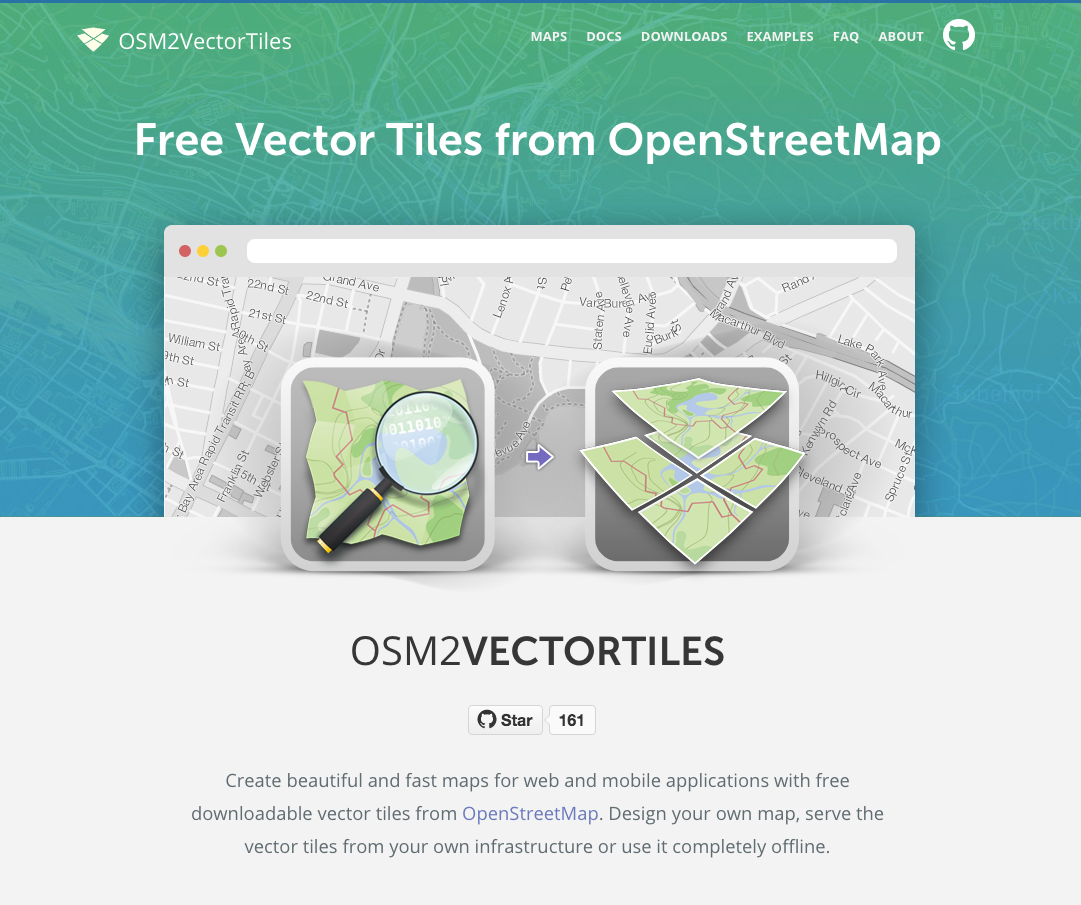
\includegraphics[width=\textwidth]{images/project_website}
\caption*{Project website \osmvt{} providing docs, downloads and examples}
\end{figure}

\endgroup

\vfill
